\documentclass[conference]{IEEEtran}
\IEEEoverridecommandlockouts

\usepackage{cite}
\usepackage{amsmath,amssymb,amsfonts}
\usepackage{graphicx}
\usepackage{textcomp}
\usepackage{xcolor}
\usepackage{hyperref}
\usepackage{booktabs}
\usepackage{array}
\usepackage{listings}
\usepackage{multirow}
\usepackage{tikz}
\usetikzlibrary{shapes.geometric, arrows.meta, positioning, fit, backgrounds}

\lstset{
  basicstyle=\ttfamily\scriptsize,
  breaklines=true,
  frame=single,
  columns=fullflexible,
  backgroundcolor=\color{gray!8}
}

\hypersetup{
  colorlinks=true,
  linkcolor=blue,
  citecolor=blue,
  urlcolor=blue
}

\def\BibTeX{{\rm B\kern-.05em{\sc i\kern-.025em b}\kern-.08em
    T\kern-.1667em\lower.7ex\hbox{E}\kern-.125emX}}

\begin{document}

\title{An End-to-End Containerized Pipeline\\for Football Event Analytics}

\author{
  \IEEEauthorblockN{Mustafa \.{I}hsan Y\"{u}ce\textsuperscript{1},
                    Hazar Utku S\"{o}zer\textsuperscript{2},
                    H\"{u}seyin Korkut\textsuperscript{3},
                    Faruk \c{C}evik\textsuperscript{4}}
  \IEEEauthorblockA{
    Department of Artificial Intelligence and Data Engineering\\
    Istanbul Technical University, Istanbul, T\"{u}rkiye\\
    \textsuperscript{1}yucem21@itu.edu.tr (150210333)\quad
    \textsuperscript{2}sozer20@itu.edu.tr (150220754)\\
    \textsuperscript{3}korkuth21@itu.edu.tr (150210314)\quad
    \textsuperscript{4}cevikf22@itu.edu.tr (150220325)
  }
}

\maketitle

%% ── 1. Executive Summary ───────────────────────────────────────────────────────
\begin{abstract}
We built a containerized data pipeline that ingests football event data from
StatsBomb and turns it into interactive dashboards. The system covers two full
tournaments: UEFA Euro 2024 (51 matches, around 188{,}000 events) and the FIFA
World Cup 2022 (64 matches, around 235{,}000 events), totaling 115 matches and
422{,}510 events. Apache Airflow orchestrates ingestion. Data is loaded into a
PostgreSQL 16 star schema with five dimension tables, five fact tables, and two
materialized views. In parallel, Apache NiFi flattens the raw JSON through a
six-processor flow and indexes it into Elasticsearch 8.12.1. Kibana hosts three
dashboards: one for each tournament with Vega-Lite charts (shot maps, xG scatter
plots, goal timelines), and a third dashboard that visualizes a simulated live
match feed. The whole stack (ten Docker services) starts with a single
\texttt{docker compose up --build}. All six required course tools are used. The
pipeline is idempotent, so re-running the DAG on already-loaded data does not
create duplicates, and Docker named volumes preserve everything between restarts.
\end{abstract}

\begin{IEEEkeywords}
data engineering, containerization, ETL pipeline, sports analytics, Docker,
Apache Airflow, Apache NiFi, Elasticsearch, PostgreSQL, Kibana, StatsBomb
\end{IEEEkeywords}


%% ── 2. Problem Statement and Motivation ────────────────────────────────────────
\section{Problem Statement and Motivation}

\subsection{Football event data is messy}

Football analytics today runs on event-level data: every pass, shot, dribble,
and carry recorded with timestamps, pitch coordinates (the StatsBomb pitch is
120m by 80m), and a long list of contextual fields. StatsBomb is one of the
biggest sports data companies, and they release a curated portion of their data
publicly under an open license \cite{statsbomb_open}. We used this data as the
input to our pipeline.

The format is not friendly. A single match file is an array of several thousand
JSON objects, one per event. Many fields are nested: \texttt{pass.end\_location}
is a two-element array of coordinates, \texttt{shot.statsbomb\_xg} sits inside
a \texttt{shot} sub-object, and player references look like
\texttt{\{"id": 12345, "name": "..."\}} instead of plain foreign keys. Different
event types carry different fields, so a pass event has no \texttt{shot} object
and vice versa. The Euro 2024 dataset is around 188{,}000 events across 51
matches; the World Cup 2022 dataset adds another 235{,}000 events across 64
matches.

\subsection{Why this is a data engineering problem}

Going from this raw JSON to dashboards involves a chain of steps: downloading
data, validating it, flattening the nested structure, loading normalized rows
into a relational database for SQL analytics, indexing flat documents into a
search engine for fast queries, and building visualizations on top. Each step
has its own failure modes and design choices that affect the next one.

We rarely got to do all of this end-to-end in earlier coursework, where each
tool was usually demonstrated by itself on a small example. Our project ties
six course tools together into a single working system that gives each tool a
real role.

\subsection{Why these two tournaments}

We picked UEFA Euro 2024 and FIFA World Cup 2022. Both are complete tournaments
in the StatsBomb open release, meaning every match is included rather than just
a sample. That matters because aggregate stats like top scorers and total xG
only make sense if the dataset is complete. Euro 2024 is also the most recent
international tournament available, and World Cup 2022 is the largest one in
the open dataset.

We initially planned to use La Liga 2015/16 as the second dataset but found out
during testing that the open release for that competition only contains around
40 cherry-picked matches with Barcelona missing entirely. Top-scorer numbers
made no sense (the leaderboard had a player from Eibar with 6 goals as the
overall top scorer), so we switched to World Cup 2022.

The two datasets do not share player rosters in any meaningful way, so we keep
them as fully separate analytical namespaces: separate Elasticsearch queries,
separate Kibana dashboards, no joins between them. If we mixed them, a player
who scored 9 goals in the World Cup (Mbapp\'e, Messi) would appear with a
combined goal count next to their zero from a tournament they never played in,
which would just be misleading.


%% ── 3. Architectural Design ────────────────────────────────────────────────────
\section{Architectural Design}

\subsection{Components}

The system has ten Docker services defined in a single
\texttt{docker-compose.yml}. They communicate over an internal bridge network
called \texttt{pipeline-net} using Docker's DNS, so no service depends on
\texttt{localhost} or the host IP. Figure~\ref{fig:arch} shows how the pieces
fit together.

\begin{figure}[ht]
\centering
\resizebox{\columnwidth}{!}{%
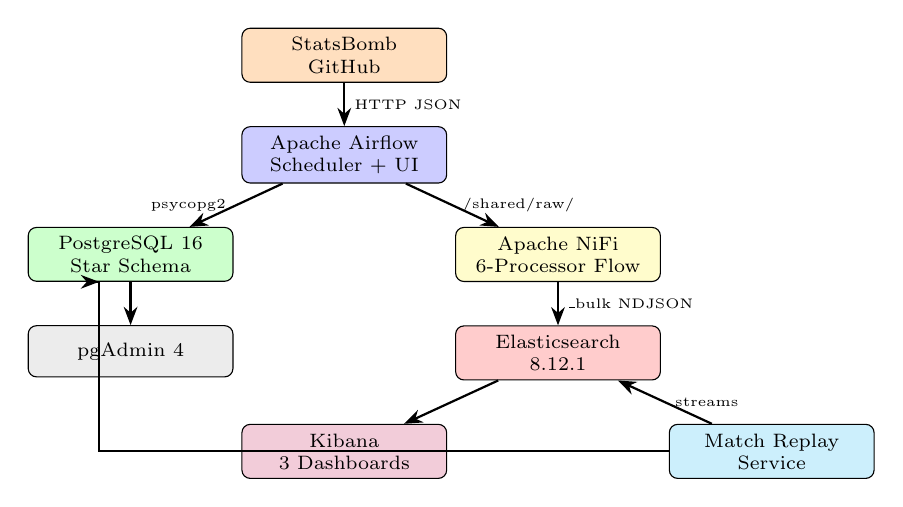
\begin{tikzpicture}[
  box/.style={draw, rounded corners=3pt, minimum width=2.6cm,
              minimum height=0.65cm, font=\scriptsize, align=center},
  arrow/.style={-Stealth, thick},
  label/.style={font=\tiny, midway},
  node distance=0.45cm and 0.3cm
]
  \node[box, fill=orange!25] (sb)   {StatsBomb\\GitHub};
  \node[box, fill=blue!20,   below=0.55cm of sb]  (af)  {Apache Airflow\\Scheduler + UI};
  \node[box, fill=green!20,  below left=0.55cm and 0.1cm of af]  (pg)   {PostgreSQL 16\\Star Schema};
  \node[box, fill=yellow!20, below right=0.55cm and 0.1cm of af] (nifi) {Apache NiFi\\6-Processor Flow};
  \node[box, fill=gray!15,   below=0.55cm of pg]  (pga)  {pgAdmin 4};
  \node[box, fill=red!20,    below=0.55cm of nifi] (es)   {Elasticsearch\\8.12.1};
  \node[box, fill=purple!20, below left=0.55cm and 0.1cm of es]  (kb)  {Kibana\\3 Dashboards};
  \node[box, fill=cyan!20,   below right=0.55cm and 0.1cm of es] (rp)  {Match Replay\\Service};

  \draw[arrow] (sb)   -- node[right,label]{HTTP JSON} (af);
  \draw[arrow] (af)   -- node[left, label]{psycopg2} (pg);
  \draw[arrow] (af)   -- node[right,label]{/shared/raw/} (nifi);
  \draw[arrow] (pg)   -- (pga);
  \draw[arrow] (nifi) -- node[right,label]{\_bulk NDJSON} (es);
  \draw[arrow] (es)   -- (kb);
  \draw[arrow] (rp)   -- node[right,label]{streams} (es);
  \draw[arrow] (rp) -| ([xshift=-0.4cm]pg.south) -- (pg);
\end{tikzpicture}%
}
\caption{System component diagram with primary data flow directions.}
\label{fig:arch}
\end{figure}

\subsection{Startup order}

The \texttt{depends\_on} block in \texttt{docker-compose.yml} controls how the
services come up. PostgreSQL has to pass its \texttt{pg\_isready} health check
before Airflow or pgAdmin start. Elasticsearch has to reach a yellow or green
cluster status before Kibana, the NiFi setup container, or the match-replay
service start. NiFi itself takes about 90--120 seconds to fully boot, so we
gave it a 120-second startup grace window before health checks kick in. The
\texttt{nifi-setup} container then polls the NiFi REST API up to 50 times (with
10-second gaps) and, once NiFi is ready, builds the processing flow and imports
the Kibana saved objects. It exits cleanly afterwards and does not restart.

\subsection{Two parallel paths}

The Airflow DAG splits into two paths that run in parallel.

The \textit{relational path} uses \texttt{statsbombpy} \cite{statsbombpy} to
load dimension tables (\textit{dim\_competitions}, \textit{dim\_matches},
\textit{dim\_teams}, \textit{dim\_players}, \textit{dim\_event\_types}) and
fact tables (\textit{fact\_events}, \textit{fact\_passes}, \textit{fact\_shots})
straight into PostgreSQL using \texttt{psycopg2} batch inserts. The materialized
views are refreshed at the end of the run so dashboard queries hit precomputed
aggregates.

The \textit{document path} downloads the raw event JSON from the StatsBomb
GitHub repo, adds \texttt{competition\_name} and \texttt{season\_name} fields
into each event before saving (this saves a join on the Elasticsearch side
later), and writes one file per match into the shared Docker volume at
\texttt{/shared/raw/}. NiFi watches this directory and processes each file
through six processors, ending with a bulk POST into Elasticsearch.

\subsection{Why this design}

We chose two stores because they are good at different things. PostgreSQL is
the source of truth and is good for normalized, multi-table SQL queries through
pgAdmin. Elasticsearch is faster for document-level lookups, full-text search,
and the spatial queries Kibana uses for shot maps and heatmaps. Kibana's
Vega-Lite charts also embed Elasticsearch aggregation queries directly, which
is much simpler than going through a server-side join.

We picked a shared Docker volume for the Airflow-to-NiFi handoff instead of
HTTP. This way Airflow does not need to know how fast NiFi is processing, the
folder acts as a natural queue, and if NiFi crashes the files are still on disk
waiting.

Idempotency was a hard requirement. Every \texttt{INSERT} in the SQL code uses
\texttt{ON CONFLICT DO NOTHING}, the download task skips files that already
exist, and the NiFi GetFile processor moves processed files to
\texttt{/shared/processed/} instead of deleting them. This means we can
re-trigger the DAG on a half-loaded dataset without producing duplicates.

We also enforced strict separation between competitions. Every Kibana
visualization includes a competition filter
(\texttt{\{"term":\{"competition\_name":"..."\}\}}) in its embedded ES query,
so no panel can accidentally show data from the wrong tournament regardless of
what the user types into the global filter bar.


%% ── 4. Tools Used and Rationale ───────────────────────────────────────────────
\section{Tools Used and Rationale}

Table~\ref{tab:tools} compares each tool we used against the main alternatives
we considered. The subsections below explain each choice in more detail.

\begin{table}[ht]
\caption{Tool Selection and Alternatives Considered}
\label{tab:tools}
\renewcommand{\arraystretch}{1.15}
\begin{tabular}{@{}p{1.5cm}p{1.5cm}p{1.5cm}p{2.6cm}@{}}
\toprule
\textbf{Tool} & \textbf{Role} & \textbf{Alternative} & \textbf{Why Chosen} \\
\midrule
Airflow & Orchestration & Prefect, Cron & DAG dependencies, retries, course tool \\
NiFi & Data flow & Logstash, Python script & Visual Jolt transforms, REST-configurable \\
PostgreSQL & Relational store & MySQL, SQLite & Materialized views, \texttt{ON CONFLICT} \\
pgAdmin & DB admin & DBeaver & Course tool, Docker-native \\
Elasticsearch & Doc store & Solr, MongoDB & Native Kibana integration, geo\_point \\
Kibana & Dashboards & Grafana, Superset & Vega-Lite, ES-native KQL filter bar \\
\bottomrule
\end{tabular}
\end{table}

\subsection{Apache Airflow}

Airflow runs the orchestration. It gives us a DAG with explicit task
dependencies, automatic retries (\texttt{retries=2},
\texttt{retry\_delay=2\,min}), and a UI we can use to monitor and re-trigger
runs. The main reason to use it over a cron job or a single Python script is
that Airflow forces task ordering: the fact-loading task literally cannot run
until the dimension-loading task has committed its rows, so we never get
foreign-key errors. Prefect and Dagster do similar things but neither is on
the course tool list. We used the LocalExecutor since we are running on a
single machine and did not need the complexity of Celery or Kubernetes.

\subsection{Apache NiFi}

NiFi handles the document path: reading raw files, transforming JSON, and
pushing batches into Elasticsearch. Its \texttt{JoltTransformJSON} processor
fits StatsBomb data really well because the JSON has up to four levels of
nesting. Our Jolt SHIFT spec maps over 40 fields declaratively, for example
turning \texttt{pass.end\_location[0]} into \texttt{pass\_end\_x}, without us
having to write Python code that walks the tree. Logstash could do similar
work but it does not have NiFi's visual flow canvas and ties more tightly to
Elasticsearch's input plugins. A custom Python script would have ended up as
a fragile field-mapping layer we would have to maintain. The whole NiFi flow
is also built automatically at startup through the REST API by our
\texttt{nifi-setup} container, so nobody has to drag and drop processors in
the UI.

\subsection{PostgreSQL 16 and pgAdmin}

We picked PostgreSQL over MySQL for three specific reasons. First,
\texttt{MATERIALIZED VIEW} with explicit \texttt{REFRESH} control: this lets
us precompute per-match and per-player stats and refresh them on demand at
the end of each DAG run. Second, the \texttt{INSERT ... ON CONFLICT DO NOTHING}
syntax: this is what makes our pipeline idempotent without us having to write
extra checks. Third, native UUID support: StatsBomb event IDs are UUIDs, and
storing them as a real \texttt{UUID} type is faster than string comparisons.
SQLite was off the table because it does not handle concurrent writes from
multiple Airflow tasks. pgAdmin gives us a graphical SQL editor we use during
the live demo to run analytical queries directly against the schema.

\subsection{Elasticsearch 8.12.1}

Elasticsearch is built around inverted indexes, which makes it very fast for
the kinds of queries Kibana sends: full-text search, term aggregations,
spatial filters. The \texttt{geo\_point} mapping on the location fields lets
us bucket shots into pitch zones for the heatmap without precomputing
anything. We mapped \texttt{player\_name}, \texttt{team\_name}, and
\texttt{competition\_name} as \texttt{text} with a \texttt{.keyword} sub-field
so we can both search and do exact-match aggregations on the same column.
Solr would have been similar but has weaker Kibana integration and a less
pleasant REST API. MongoDB does not come with dashboards, so we would have
needed another tool on top.

\subsection{Kibana 8.12.1}

Kibana talks to Elasticsearch directly and supports Vega-Lite custom charts,
where the Elasticsearch aggregation query is embedded right into the chart
spec. This is how we built the xG scatter plot, the shot heatmap, the
goals-by-minute area chart, and the top-scorer bar without setting up a
separate visualization service. Grafana has Elasticsearch support but its
focus is metrics and time-series, and it does not render Vega-Lite. Apache
Superset can render Vega-Lite but needs its own backend database. Kibana also
gives us the KQL filter bar at the top of each dashboard, which lets users
narrow down the data interactively without us having to rewrite each chart.


%% ── 5. Implementation Details ──────────────────────────────────────────────────
\section{Implementation Details}

\subsection{PostgreSQL star schema}

The schema follows a standard star pattern. Table~\ref{tab:schema} lists the
tables and their main columns.

\begin{table}[ht]
\caption{PostgreSQL Schema Summary}
\label{tab:schema}
\renewcommand{\arraystretch}{1.1}
\begin{tabular}{@{}lll@{}}
\toprule
\textbf{Table} & \textbf{Type} & \textbf{Key Columns} \\
\midrule
dim\_competitions & Dimension & competition\_id (PK), season\_id \\
dim\_matches & Dimension & match\_id (PK), competition\_id (FK) \\
dim\_teams & Dimension & team\_id (PK), team\_name \\
dim\_players & Dimension & player\_id (PK), player\_name \\
dim\_event\_types & Dimension & type\_id (PK), type\_name \\
fact\_events & Fact (central) & event\_uuid (PK), match\_id, player\_id, \\
             &               & period, minute, location\_x/y \\
fact\_passes & Fact & event\_uuid (FK), pass\_length, pass\_angle, \\
             &      & pass\_end\_x/y, pass\_outcome \\
fact\_shots & Fact & event\_uuid (FK), shot\_xg, shot\_outcome, \\
            &      & shot\_technique, first\_time \\
fact\_dribbles & Fact & event\_uuid (FK), dribble\_outcome \\
fact\_carries & Fact & event\_uuid (FK), carry\_end\_x/y \\
mv\_match\_summary & Mat. View & total\_events, total\_shots, total\_xg \\
mv\_player\_stats & Mat. View & goals, total\_xg, total\_passes \\
\bottomrule
\end{tabular}
\end{table}

We added seven B-tree indexes for the queries we run most often: lookups by
\texttt{match\_id}, \texttt{player\_id}, \texttt{team\_id}, and
\texttt{type\_id} on \textit{fact\_events}, a composite index on
\texttt{(period, minute)} for time-window queries, and outcome indexes on
\textit{fact\_shots} and \textit{fact\_passes}. The \texttt{event\_uuid}
column is stored as a real UUID type rather than a string.

The unique constraint on \texttt{(match\_id, event\_index)} in
\textit{fact\_events} doubles as our idempotency key.
\texttt{ON CONFLICT (match\_id, event\_index) DO NOTHING} means re-running the
DAG never produces duplicates.

\subsection{Airflow DAG}

The DAG is called \texttt{statsbomb\_football\_pipeline}, has
\texttt{schedule="@once"} and \texttt{catchup=False}, and contains seven tasks
arranged into two branches:

\begin{lstlisting}
setup_directories >> [load_dimensions, download_raw_events]
load_dimensions   >> load_fact_tables >> refresh_views
download_raw_events >> trigger_nifi >> verify_elasticsearch
\end{lstlisting}

\texttt{setup\_directories} creates the three shared paths
(\texttt{/shared/raw/}, \texttt{/shared/processed/},
\texttt{/shared/nifi\_trigger/}) and gates everything else. After that the two
branches run in parallel.

\texttt{load\_fact\_tables} loops over all 115 matches and skips any
\texttt{match\_id} that already has rows in \texttt{fact\_events} (using a
quick \texttt{SELECT 1 ... LIMIT 1} check). For new matches it inserts events
in batches of 500 using \texttt{psycopg2.extras.execute\_batch}, then inserts
passes and shots in their own batch calls inside the same transaction.

\texttt{download\_raw\_events} fetches the event JSON for each match from the
StatsBomb GitHub raw URL, injects the \texttt{competition\_name} field into
every event so NiFi can pass it through to Elasticsearch later, and saves it
to \texttt{/shared/raw/\{match\_id\}.json}. Files that already exist are
skipped, which makes re-runs both safe and fast.

\texttt{verify\_elasticsearch} polls the \texttt{\_count} endpoint up to twelve
times with 30-second gaps. It is our automated data-quality check: the DAG
does not consider itself done until at least one document is in the index.
The final document count gets logged.

\subsection{NiFi flow}

The NiFi flow is built from scratch by the \texttt{nifi-setup} container at
first launch through the NiFi REST API, so nobody has to set it up by hand in
the UI. It is six processors connected in a line, all inside a single process
group called \textit{StatsBomb Football Pipeline}. Table~\ref{tab:nifi} lists
each one.

\begin{table}[ht]
\caption{NiFi Processor Configuration}
\label{tab:nifi}
\renewcommand{\arraystretch}{1.1}
\begin{tabular}{@{}p{2.0cm}p{5.3cm}@{}}
\toprule
\textbf{Processor} & \textbf{Role and Key Configuration} \\
\midrule
GetFile & Polls \texttt{/shared/raw/} every 1\,s; batch size 5; min file age
          2\,s to avoid reading partially written files; moves consumed files to
          \texttt{/shared/processed/} \\[3pt]
SplitJson & JSON path \texttt{\$.*}; splits the top-level array into one
            FlowFile per event; original and failure relationships
            auto-terminated \\[3pt]
JoltTransformJSON & Jolt SHIFT chain spec (external JSON file); maps 40+
                    nested StatsBomb fields to flat keys, e.g.\ \texttt{location[0]}
                    $\rightarrow$ \texttt{location\_x},
                    \texttt{shot.statsbomb\_xg} $\rightarrow$ \texttt{shot\_xg} \\[3pt]
ReplaceText & Regex Replace on entire text; prepends the ES bulk action header
              \texttt{\{"index":\{"\_index":"football\_events"\}\}} before each
              document \\[3pt]
MergeContent & Bin-packing strategy; minimum 1, maximum 100 FlowFiles per bin;
               max bin age 10\,s; produces a single NDJSON payload per batch \\[3pt]
InvokeHTTP & POST to \texttt{http://elasticsearch:9200/\_bulk}; content-type
             \texttt{application/x-ndjson}; connection timeout 5\,s; read
             timeout 30\,s; all response relationships auto-terminated \\
\bottomrule
\end{tabular}
\end{table}

The 2-second minimum file age on GetFile prevents a race condition where NiFi
starts reading a file before Airflow has finished writing it. The batch size
of 100 on MergeContent is a tradeoff: bigger batches mean fewer HTTP calls
into Elasticsearch, but smaller batches mean events show up in the dashboard
sooner.

\subsection{Jolt spec}

The Jolt SHIFT spec flattens StatsBomb's nested JSON. It renames
\texttt{id} to \texttt{event\_id}, lifts \texttt{type.name} to
\texttt{type\_name}, \texttt{team.name} to \texttt{team\_name},
\texttt{player.name} to \texttt{player\_name}, and splits \texttt{location[0]}
and \texttt{location[1]} into \texttt{location\_x} and \texttt{location\_y}.
Pass fields (\texttt{pass.end\_location[0/1]}, \texttt{pass.length},
\texttt{pass.angle}, \texttt{pass.outcome.name}) and shot fields
(\texttt{shot.statsbomb\_xg}, \texttt{shot.outcome.name},
\texttt{shot.technique.name}, \texttt{shot.body\_part.name}) all get promoted
to top-level keys the same way. The \texttt{competition\_name} and
\texttt{match\_id} fields injected by Airflow during download are passed
through unchanged.

Some event types we did not map explicitly (\texttt{50\_50},
\texttt{ball\_receipt}, \texttt{goalkeeper}) still get indexed, but with their
original nested structure. Their fields are searchable but cannot be used in
Kibana aggregations until we extend the spec.

\subsection{Elasticsearch index design}

The \texttt{football\_events} index uses an explicit mapping defined in
\texttt{elasticsearch/events\_mapping.json} and applied at index creation by
the \texttt{nifi-setup} container. Key choices:

\begin{itemize}
  \item \texttt{location\_x} and \texttt{location\_y} are \texttt{float} so we
        can do range queries for pitch-zone filters.
  \item \texttt{competition\_name}, \texttt{player\_name}, \texttt{team\_name},
        and \texttt{type\_name} are \texttt{text} with a \texttt{.keyword}
        sub-field. Text supports search, keyword supports exact-match
        \texttt{terms} aggregations (which is what the top-scorer chart needs).
  \item \texttt{shot\_xg} is a \texttt{float} for sum aggregations.
  \item \texttt{match\_id} is an \texttt{integer} for term filters in the
        replay dashboard.
  \item \texttt{minute} is an \texttt{integer} for the histogram aggregation
        that powers the goals-by-minute area chart (5-minute bins).
\end{itemize}

The match-replay service creates a second index, \texttt{football\_replay},
with the same field types plus a \texttt{replay\_timestamp} field that the
Live Replay dashboard filters on.

\subsection{Kibana dashboards}

There are three dashboards, all imported automatically at startup. The two
competition dashboards (UEFA Euro 2024, FIFA World Cup 2022) have the same
panel layout but each panel runs a competition-scoped Elasticsearch query, so
the two dashboards are completely separate. Each one has twelve panels in
four rows:

\begin{enumerate}
  \item \textit{Five KPI tiles}: Matches Played, Goals, Shots, Total xG, Total
        Passes. Each tile is a Kibana Metric visualization with a KQL filter
        on \texttt{competition\_name} and a single max or count aggregation.
  \item \textit{Top Scorers bar chart and xG vs Goals scatter chart}. Both are
        Vega-Lite. The top scorers chart uses a nested \texttt{terms}
        aggregation to count goals per player and pull each player's main team
        for color coding. The scatter plots each player at (total\_xg, goals);
        if a player is above the \(y=x\) line they overperformed their xG.
  \item \textit{Top Teams by xG bar and Goals by Minute area chart}. The bar
        ranks teams by their summed \texttt{shot\_xg}. The area chart bins
        goal events into 5-minute intervals and stacks them by team.
  \item \textit{Shot heatmap, Player table, and Interactive shot map}. The
        heatmap divides the pitch into a 24-by-16 grid. The player table is a
        Kibana data-table ranking the top 20 players by xG. The shot map is a
        Vega-Lite scatter on a pitch overlay where each shot is a circle sized
        by xG, and the KQL filter bar lets you isolate a single team.
\end{enumerate}

All Vega-Lite specs use \texttt{"autosize": "none"} with explicit widths and
heights so they do not reflow inside the Kibana grid. Competition isolation
is enforced inside the embedded query: each spec includes a \texttt{must}
clause with a \texttt{term} filter on \texttt{competition\_name}, which means
no panel can ever leak the other tournament's data into view, no matter what
the user does with the global filter bar.


%% ── 6. Evaluation ──────────────────────────────────────────────────────────────
\section{Evaluation}

\subsection{Volume and correctness}

After a full run, Elasticsearch holds 422{,}510 documents in
\texttt{football\_events}: 187{,}858 from Euro 2024 and 234{,}652 from World
Cup 2022. We checked these totals against StatsBomb's published per-match
event counts using competition-scoped \texttt{\_count} queries:

\begin{lstlisting}
GET /football_events/_count
{"query":{"term":{"competition_name":"UEFA Euro"}}}
\end{lstlisting}

The PostgreSQL \texttt{fact\_events} row count matches the Elasticsearch
document count exactly: 422{,}510 events in both stores, with the same per-
competition split. Both paths are sourced from the same raw StatsBomb JSON, so
they should agree row-for-row, and they do.

We also checked correctness against public tournament records. The World Cup
2022 dashboard shows Mbapp\'e and Messi tied at 9 goals each, including
penalty-shootout goals (StatsBomb counts these under \texttt{shot\_outcome =
'Goal'}, which inflates the figures above the official FIFA Golden Boot
record of 8 for Mbapp\'e). The Euro 2024 top scorer in our dashboard is a
five-way tie at 3 goals, also consistent with public stats. Total xG
across all World Cup matches (\texttt{SELECT SUM(shot\_xg) ...}) lands in the
expected range for the tournament.

\subsection{Idempotency}

We triggered the Airflow DAG twice in a row on the same data. On the second
run, all the \texttt{download\_raw\_events} iterations exited early (file
already present), all the \texttt{load\_fact\_tables} iterations skipped their
match (rows already there), and \texttt{refresh\_views} ran normally.
PostgreSQL row counts were the same before and after. NiFi found no new files
in \texttt{/shared/raw/} and did nothing.

\subsection{Performance}

Table~\ref{tab:perf} shows timings we measured on a 16\,GB MacBook on a
100\,Mbps connection.

\begin{table}[ht]
\caption{Pipeline Performance Measurements}
\label{tab:perf}
\renewcommand{\arraystretch}{1.1}
\begin{tabular}{@{}lrr@{}}
\toprule
\textbf{Stage} & \textbf{Duration} & \textbf{Notes} \\
\midrule
docker compose up (services start) & 3--5 min & NiFi JVM dominates \\
download\_raw\_events (115 matches) & 4--6 min & ~2 MB/match from GitHub \\
load\_fact\_tables (115 matches) & 8--12 min & psycopg2 batch inserts \\
NiFi Elasticsearch indexing & 10--15 min & 100-event batches \\
\textbf{Total cold-start to dashboards} & \textbf{20--30 min} & \\
\midrule
Kibana dashboard load (warm cache) & $<$2 s & All panels \\
ES \_count query & $<$100 ms & \\
PostgreSQL mat.\ view query & $<$300 ms & mv\_player\_stats \\
\bottomrule
\end{tabular}
\end{table}

NiFi indexing was much slower at first (15-second poll, batch size 1). After
we tuned GetFile to a 1-second poll with batch size 5, the queue drained in
about 12 minutes instead of 28.

\subsection{Failure recovery}

We tested three failure scenarios.

When PostgreSQL was restarted mid-ingestion, \texttt{load\_fact\_tables}
failed with a connection error. Airflow retried after 2 minutes, the task
picked up from the first unloaded match (the idempotency check skipped the
already-committed ones), and no duplicates appeared.

When Elasticsearch was restarted, Kibana panels showed connection errors.
Once Elasticsearch came back up and passed its health check, Kibana
reconnected automatically and all panels filled in from the persisted
\texttt{es-data} volume.

When NiFi was restarted, it reloaded the previously built flow from
\texttt{nifi-conf}. Files still in \texttt{/shared/raw/} (not yet moved to
\texttt{/shared/processed/}) got picked up by GetFile and indexed normally.


%% ── 7. Limitations and Future Work ────────────────────────────────────────────
\section{Limitations and Future Work}

\subsection{Jolt coverage is incomplete}

Our Jolt spec covers the event sub-types that matter most for analytics
(shots, passes, carries, dribbles, pressures). Events with more complex
nesting — \texttt{50\_50} outcomes that reference two players, goalkeeper
saves with dive position fields, \texttt{ball\_receipt} outcomes — get indexed
with their original structure, which means Kibana cannot run \texttt{terms}
or \texttt{histogram} aggregations on those fields. Extending the spec is not
hard, but it does mean reading StatsBomb's documentation for each sub-type
and adding the right SHIFT entries.

\subsection{No automated tests}

We do not have unit or integration tests. Data quality checking is limited to
\texttt{verify\_elasticsearch} and our own visual inspection of the
dashboards. Adding \texttt{pytest} fixtures with a small synthetic event
dataset and \texttt{great-expectations} checks against the PostgreSQL fact
tables would be a real improvement and would make schema or transform changes
much safer.

\subsection{Resource use}

The full stack uses around 6--8\,GB of RAM at idle: roughly 200\,MB for
PostgreSQL, 512\,MB to 1\,GB for Elasticsearch, the same for NiFi, around
600\,MB for Kibana, and 400\,MB for Airflow's webserver and scheduler. On
8\,GB machines you have to drop the JVM heaps for NiFi and Elasticsearch in
the \texttt{.env} file. A lighter-weight mode that pre-downloads a small
sample dataset would make the demo accessible on weaker hardware.

\subsection{Batch ingestion only}

The match-replay service simulates live data by streaming pre-loaded events
at 30x speed. A genuinely live pipeline would consume events as they happen
through a message broker like Kafka, with NiFi as a Kafka consumer instead of
a file watcher. That would turn the system into real-time ingestion without
needing to change the Elasticsearch or Kibana side.

\subsection{Commit history}

Our git history is not evenly distributed across the team. A lot of the
system was built in pair-programming sessions on a single machine, so
commits are concentrated on a few accounts. Next time we should use feature
branches and individual pull requests to make contributions visible.

\subsection{Abstract vs final dataset}

We submitted the abstract a week before the final deadline, and at that point
our second dataset was La Liga 2015/16. While testing we found out that the
StatsBomb open release for that competition only includes around 40 matches
(a curated sample, with Barcelona missing), which made the top-scorer numbers
nonsensical. We replaced it with FIFA World Cup 2022, which is a complete
64-match dataset. So the abstract has different match and event totals than
this report does. The architecture, tools, and design decisions did not
change — only the dataset.


%% ── 8. AI Usage Declaration ────────────────────────────────────────────────────
\section{AI Usage Declaration}

\textbf{Tool used:} Claude Code (Anthropic, \textit{claude-sonnet-4-6}).

\textbf{Purpose:} We used Claude Code as a coding and reasoning assistant
during development. It helped with implementation work like writing
boilerplate code, getting configuration syntax right (NiFi processor
properties, Elasticsearch mappings, Docker Compose health checks), debugging
Kibana Vega-Lite errors, and thinking through technical issues we hit during
integration. The system architecture, project plan, dataset choice, tool
selection, and engineering decisions were ours. Claude Code's role was to
help us implement and debug the system we had already designed, not to design
it.

\textbf{Validation:} We tested the full pipeline end-to-end multiple times in
different conditions, including normal runs, re-triggered DAG runs, and
restarts of individual services. Every AI-assisted output was read,
understood, and verified by a team member before being committed. We checked
correctness against known ground truth — tournament top-scorer records,
published match counts, expected event totals — instead of trusting generated
code on its face.


%% ── 9. Individual Contribution Table ──────────────────────────────────────────
\section*{Appendix: Individual Contribution Table}

\begin{table}[ht]
\caption{Individual Team Contributions}
\label{tab:contrib}
\renewcommand{\arraystretch}{1.15}
\begin{tabular}{@{}p{2.1cm}p{5.6cm}@{}}
\toprule
\textbf{Member} & \textbf{Primary Contributions} \\
\midrule
Mustafa \.{I}hsan Y\"{u}ce (150210333) &
  Docker Compose service definitions and health-check configuration;
  Elasticsearch index mapping design; Kibana dashboard layout,
  panel arrangement, and saved-objects import automation. \\[4pt]
Hazar Utku S\"{o}zer (150220754) &
  Airflow DAG design and implementation; PostgreSQL star-schema design
  and SQL queries; NiFi setup script and REST flow builder;
  system integration, debugging, and dataset selection. \\[4pt]
H\"{u}seyin Korkut (150210314) &
  Match replay streaming service; Jolt SHIFT transformation
  specification; Kibana Vega-Lite visualization specifications
  (shot map, xG scatter, goals timeline, heatmap). \\[4pt]
Faruk \c{C}evik (150220325) &
  StatsBomb data acquisition and statsbombpy integration;
  README and project documentation; evaluation, correctness
  testing, and performance measurements. \\
\bottomrule
\end{tabular}
\end{table}


%% ── References ─────────────────────────────────────────────────────────────────
\begin{thebibliography}{00}

\bibitem{statsbomb_open}
StatsBomb, ``StatsBomb Open Data,'' GitHub repository, 2024.
[Online]. Available: \url{https://github.com/statsbomb/open-data}

\bibitem{statsbombpy}
StatsBomb, ``statsbombpy: Python package for StatsBomb open data,'' GitHub, 2024.
[Online]. Available: \url{https://github.com/statsbomb/statsbombpy}

\bibitem{airflow_docs}
Apache Software Foundation, ``Apache Airflow Documentation,'' 2024.
[Online]. Available: \url{https://airflow.apache.org/docs/}

\bibitem{nifi_docs}
Apache Software Foundation, ``Apache NiFi Documentation,'' 2024.
[Online]. Available: \url{https://nifi.apache.org/docs.html}

\bibitem{jolt_spec}
Bazaarvoice, ``Jolt: JSON to JSON transformation library,'' GitHub, 2023.
[Online]. Available: \url{https://github.com/bazaarvoice/jolt}

\bibitem{es_docs}
Elastic, ``Elasticsearch Reference 8.12,'' 2024.
[Online]. Available: \url{https://www.elastic.co/guide/en/elasticsearch/reference/8.12/}

\bibitem{kibana_vega}
Elastic, ``Vega and Vega-Lite in Kibana,'' 2024.
[Online]. Available: \url{https://www.elastic.co/guide/en/kibana/current/vega.html}

\bibitem{pg16_docs}
The PostgreSQL Global Development Group, ``PostgreSQL 16 Documentation,'' 2024.
[Online]. Available: \url{https://www.postgresql.org/docs/16/}

\bibitem{docker_compose}
Docker, Inc., ``Docker Compose Documentation,'' 2024.
[Online]. Available: \url{https://docs.docker.com/compose/}

\bibitem{vegalite}
B.~Satyanarayan, D.~Moritz, K.~Wongsuphasawat, and J.~Heer,
``Vega-Lite: A Grammar of Interactive Graphics,''
\textit{IEEE Trans.\ Visualization \& Comp.\ Graphics}, vol.~23, no.~1,
pp.~341--350, Jan. 2017.

\bibitem{statsbomb_spec}
StatsBomb, ``StatsBomb Event Specification,'' Technical Documentation, 2024.
[Online]. Available: \url{https://github.com/statsbomb/open-data/tree/master/doc}

\bibitem{docker_health}
Docker, Inc., ``HEALTHCHECK instruction in Dockerfile,'' 2024.
[Online]. Available: \url{https://docs.docker.com/reference/dockerfile/#healthcheck}

\end{thebibliography}

\end{document}
